\section{Development Method and Organisational Tools}
The entire GIRAF project met to discuss the information gathered from last years reports, to discuss pros and cons of the process they used.
Last year's reports recomended to change different aspects of their development process, and their advice has been taken into consideration.
This section will first present the chosen development method as has been chosen at this meeting, and will finally present the tools that will accomodate the development method.


\subsection*{Development Method of the Multi-Project}
The previous semester of the GIRAF project used the agile development method \textit{scrum of scrum}, which is a scaled version of \textit{scrum}.
This is also the choice for the multi-project of 2016, but where as last year they had three-layers of scrum, as the multi-project was seperated into three further sub-projects:
\begin{itemize}
	\item Applications
	\item Database
	\item Build & Deployment
\end{itemize}

This is changed for the multi-project of 2016, as many of the reports from last year recomended this change, such that any group would be able to work on any tasks which occur during the project.

In order to explain how scrum of scrum works, a brief explanation of scrum is now presented.
This is in turn also how we will be working internally in group SW618F16. 


\subsubsection*{Scrum}

We use parts of the version of scrum as defined by Sommerville in his book, Software Engineering in chapter three \cite{SEBOOK}.
The parts used are presented here.

\begin{description}
	\item[Daily scrum] Everyday we start out by having a daily scrum, which is a meeting where each person in the group is asked the following questions:
		\begin{itemize}
		    \item What did you do yesterday? 
			\item What will you do today?
			\item What obstacles are in your way or slowing you down?		
		\end{itemize}
		This helps make sure that all group members know what each other are doing, while also giving an opportunity to ask for help if needed.

	\item[Sprints] A sprint is a working period where the group sets out to complete different tasks before the sprint end. 
	\item[Product Backlog] A product backlog is a list of tasks which are to be done in order for the project to be complete. 
	It replaces traditional requirements lists, and can develop throughout development, more tasks can be added throughout the project.
	When a sprint starts, some of these tasks are chosen by the group, and these tasks are then to be estimated in half-days, and completed before the sprint end.
	All tasks on the backlog are written in the form of user stories like this:``As a <type of user>, I want <some goal> so that <some reason>''.
	\item[Sprint Backlog] A sprint backlog contains the tasks chosen from the product backlog by the development team to be completed in the sprint.
	As these tasks are chosen, it is not allowed to add more tasks during this period.
	If it is discovered after estimating the tasks, that there is simply too much work to be done in the sprint, it is okay to contact the scrum master to reduce the workload.
	\item[Scrum Master] The scrum master is a role of one of the developers of the project, it is the scrum masters job to make sure that the development team uses scrum correctly, and also helps the product owner organising the product back-log.
	\item[Product Owner] The product owner is another role, which deals with understanding what the customer wants.
	The product owner is also in charge of the product backlog, and makes sure to prioritize the tasks here, and makes sure that the tasks are understandable such that it is easy for a developer to proceed with the development of the task.
	\item[Scrum Board] A scrum board is a board which contains all tasks from the sprint-backlog.
	These tasks can have different sub-tasks, and these are then moved from different columns depending on where they are currently recide in development.
	They can be in four different columns:
	\begin{itemize}
		\item Todo
		\item Doing
		\item Review
		\item Done
	\end{itemize}
	The scrum board works well to make sure that progress is visible, and to show what different tasks are currently being worked on.
	\item[Burndown Chart] The burndown chart makes gives estimates on the progress of a sprint, by calculating the total number of half-days needed to complete the tasks on the sprint-backlog, and as such requires that all tasks in the sprint backlog are time estimated.
	At every daily scrum all time estimates of the completed tasks are summed, and a line is drawn on the chart showing the progress of the tasks.
	The chart has a tendency line which shows how progress should be coming along, and groups cna then track if they are ahead or behind according to their estimated development times of their tasks.
	\todo[inline]{Er stadig i tvivl om der er beskrevet nok, i det flg. afsnit skal der stå noget med hvordan vores metode ovenfor her hænger sammen med multi-projekt. - Soren}
\end{description}

All these tools define the scrum method we use in our group, they are not independent of the scrum of scrum which is used in the multi-project, which will be explained next.

The scrum of scrum consists of multiple groups, all using scrum, and then having ambassadors from every group meet and do the scrum meetings \cite{SCRUMBOOK}.
The structure of the scrum of scrum can be seen on \myref{fig:scrumofscrum}

\begin{figure}
\centering
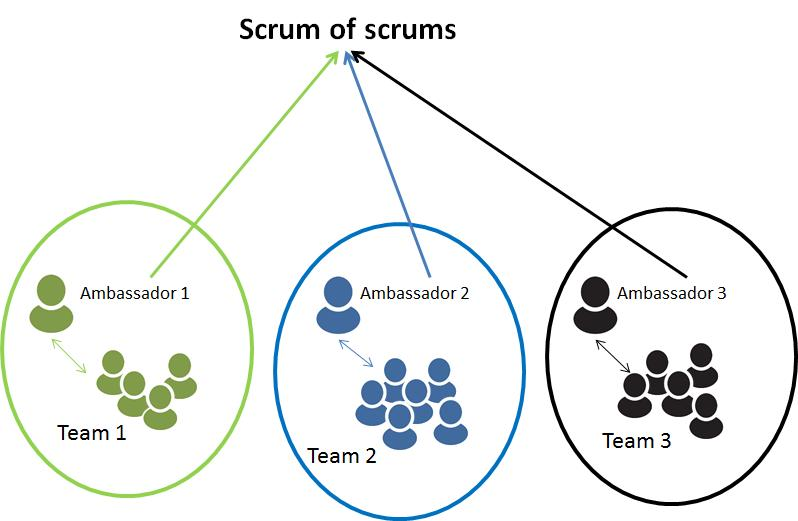
\includegraphics[scale=0.4]{figures/scrumofscrum.png}
\caption{The structure of scrum of scrum. Figure from \cite{scrumofscrumfigure}.}
\label{fig:scrumofscrum}
\end{figure}

Every group will perform a daily scrum individually, and the multi-group will perform a scrum meeting answering the same questions as one would at daily scrum but instead it is just the ambassadors from each group at this scrum meeting, whom then speak on the group's behalf.
According to MountainGoatSoftware it is not necesary to have every day, and many organisations have them two to three times a week instead. \footnote{https://www.mountaingoatsoftware.com/agile/scrum/team}
For the GIRAF project 2016, we have chosen to have one weekly scrum every wednesday instead.
The reasoning for this is that, the reports last year complained about having too many meetings, and while many organisations might have two to three a week, these organisations do not have courses to attend to, which also require a lot of time.
As the scrum of scrum meetings are held weekly the questions asked at these meeting change to asking:``...since last we met?'' etc.
There are 4 other meetings than the weekly scrum of scrums specified for the multi-project:

\begin{description}
	\item[Sprint Planning] This meeting is held at the start of a sprint.
	The sprint planning meeting is where the tasks from the product backlog will be chosen by all groups to put on their own sprint backlog.
	This means that the multi-project has a single product backlog for the multi-project, which is where all tasks come from.
	\item[Sprint Retrospective] The sprint retrospective has the job of reviewing and improving the development process. 
	This is where any issues with the process is brought up in order to improve upon the process of the project.
	\item[Sprint Review] The customers attend the sprint review meeting so we can show them the progress of the applications, to gain valuable feedback, to create new tasks, and to help prioritize the tasks. 
	\item[Presentations] Sometimes a group has something important to present to the rest of the groups, and therefore a presentation will be made to inform the other groups of the news.
\end{description}

Each sprint will be approximately 3 weeks, which gives time for approximately 4 sprints throughout the project.
At the start of each sprint the sprint planning meeting is held, afterwards the groups will estimate their chosen tasks.
When the sprint is over the sprint retrospective it held, and finally the sprint review.
The last two meetings might interchange, depending on the availability of the customers.


The scrum master of the multi-project will be group SW613F16, and they are the ones to make sure the other groups of the project adhere to the specified process.
The scrum master is one of many areas of responsibility given to the groups this semester, which will be further explained in the next section.


\subsubsection*{Areas of Responsibility}
The areas of responsibility are organisational and technical aspects of development that may require attention but are not necessarily directly linked to the software itself.
The use of scrum dictates that a project owner and a scrum master exists, as the scrum is composed of groups, these roles will be assigned to groups as areas of responsibility.
Furthermore the servers, the database and the automated building and testing tool Jenkins, has according to the papers read, often caused trouble so these will also serve as areas of responsibility. 
According to previous papers these groups also have a great deal of interaction, in order to reduce the time spent explaining the issue to other groups these areas will all be handled by the same group, as it happens all the areas is far too big a workload for a single group, thus two groups share these responsibilities.
From the previous papers it is evident that their work flow did not include a formal or even uniform way of documentation or even a consistent coding style.
As such documentation and unit/integration testing are also established as areas of responsibility.
We got the responsibility for one of these; documentation. 
This entails that we are to set up guidelines for the rest of the multi-project to follow, and to ensure they follow these guidelines.
Further areas of responsibility are derived largely from suggestions or positive feedback from the read papers, these include graphics, usability tests, security and social events/HR.
\info[inline]{jeg oververjer at stille alle op som punktform og forklare dem men ved ikke om det bliver for meget? - Marc. Jeg syntes en ``description'' kunne gøre godt her, så undgår man at det bliver rodet. - Troels Hvis vi gør det, skal det hele skrives om, og så forsvinder "historien" i teksten. - Søren}

\subsubsection*{Development and Organisational Tools}
Previously the project have used the project management tool Redmine.
However an opinion that is mostly consistent throghout all the papers from the previous semester is that Redmine should be replaced as it, according to last years students, is not a good tool.
Redmine offers tools for communication, calenders, documentation, issue tracking, a wiki and more.
The primary issue with Redmine according to last years students refer to its lackluster communication solution.
As this is a problem stated throughout a majority of the papers the web application Slack is used as the communication tool between the groups involved in development.
Furthermore it was decided at the initial meeting to replace Redmine, with another software development tool: Phabricator, an open source, software development and project management platform. 
As Phabricator is still an unfamiliar tool issues may arise, however from the initial overview it seems to be geared towards agile development with applications specific to user stories and backlog tracking.
The workflow established for Phabricator is also very geared towards code review and documentation, something the groups agree seems very lackluster and should have more focus this semester.
For more information about Phabricator visit their website at \cite{phabricatorWebsite}.
Lastly with scrum meetings happening on a weekly basis a shared Google Docs folder contains all agendas and summaries from meetings.
Furthermore, while there is a primary rapporteur for each meeting, Google Docs allows everyone to pitch in for both the agenda and the summary which in turn means that if someone is not satisfied with the information in the summary, they can also add more information in real-time.

\kim{Når man har cites der bare er links så fortrækker jeg at i bruger footnotes.}